\documentclass[man]{apa7}

%% Some pieces required from the pandoc template
\providecommand{\tightlist}{%
  \setlength{\itemsep}{0pt}\setlength{\parskip}{0pt}}

\usepackage[T1]{fontenc}
\usepackage[utf8]{inputenc}

% Pandoc citation processing
\newlength{\csllabelwidth}
\setlength{\csllabelwidth}{3em}
\newlength{\cslhangindent}
\setlength{\cslhangindent}{1.5em}
% for Pandoc 2.8 to 2.10.1
\newenvironment{cslreferences}%
  {}%
  {\par}
% For Pandoc 2.11+
\newenvironment{CSLReferences}[3] % #1 hanging-ident, #2 entry spacing
 {% don't indent paragraphs
  \setlength{\parindent}{0pt}
  % turn on hanging indent if param 1 is 1
  \ifodd #1 \everypar{\setlength{\hangindent}{\cslhangindent}}\ignorespaces\fi
  % set entry spacing
  \ifnum #2 > 0
  \setlength{\parskip}{#2\baselineskip}
  \fi
 }%
 {}
\usepackage{calc} % for calculating minipage widths
\newcommand{\CSLBlock}[1]{#1\hfill\break}
\newcommand{\CSLLeftMargin}[1]{\parbox[t]{\csllabelwidth}{#1}}
\newcommand{\CSLRightInline}[1]{\parbox[t]{\linewidth - \csllabelwidth}{#1}}
\newcommand{\CSLIndent}[1]{\hspace{\cslhangindent}#1}


\title{The Structure of Developmental Variation in Early Childhood}
\shorttitle{Structure of development}

\author{Benjamin A. Stenhaug\textsuperscript{1}, Nilam Ram\textsuperscript{2}, Michael C. Frank\textsuperscript{2}}
\date{}
\affiliation{\vspace{0.5cm}\textsuperscript{1} The Graduate School of Education, Stanford University\\\textsuperscript{2} Department of Psychology, Stanford University}

\leftheader{Weiss}

\abstract{Do children's abilities develop in tandem or on their own separate
timetables? Piaget proposed that development proceeded globally through
stages; more recent theories view development as more modular with
different abilities developing independently and on different
time-scales. The developmental differentiation hypothesis suggests that
the structure of a child's development is unitary early in infancy but
becomes more complex with age. Despite an abundance of theoretical interest in this
question, there is little empirical work on the macrostructure of
developmental changes in early childhood. We investigate this structure
using two large datasets of parent-reported developmental milestones.
Applying item response theory models, we find that variation in development across
infancy and early childhood is multidimensional. Consistent with the
differentiation hypothesis, differences among older children are better
described by higher-dimensional models. In addition, in longitudinal data, we find that, within-person changes in underlying abilities are highly
coupled early in life but their coupling decreases by age 12 months. Our work
provides a model-based method for linking holistic descriptions of early
development to basic theoretical questions about the nature of change in
childhood.

\hypertarget{sig}{%
\section{Significance Statement}\label{sig}}

How do children vary? Do some children develop globally faster or slower than others, or is variation more discrete (e.g., in motor or language skill)? Variation between children has
often been assumed to be unifactorial or multifactorial without formal
evaluation. Our work here uses psychometric modeling and big-data
approaches to evaluate this dimensionality empirically. We find evidence for multidimensionality, and further evidence that this dimensionality increases with age. This work implies that measures of developmental variation should move
beyond assumptions that differences and progression of children's
development can be represented as a homogenous process, and toward
multi-dimensional representations of within-person change.}

\authornote{
The research reported here was supported by the Institute of Education Sciences, U.S. Department of Education, through Grant R305B140009 to the Board of Trustees of the Leland Stanford Junior University. The opinions expressed are those of the author and do not represent views of the Institute or the U.S. Department of Education. Correspondence concerning this article should be addressed to Benjamin A. Stenhaug at \href{mailto:benastenhaug@gmail.com}{\nolinkurl{benastenhaug@gmail.com}}
}

\begin{document}
\maketitle

\hypertarget{intro}{%
\section{Introduction}\label{intro}}

How do young children grow and change? Is child development a single
unified process or a host of different processes, each with its own
constraints and timescale? Piaget famously proposed a stage theory in
which many seemingly distinct mental processes developed in concert
through a common set of operational stages (1). In contrast, modern
theories propose that there are different facets of children's mental
life and that these facets each develop on their own timetable (2). And attesting to a folk theory of developmental multi-dimensionality, the
grandmother of one author was known to assert that
``children either walk early or else they talk early.''

A theoretical and practical understanding of how children grow and change
provides the underpinning for parents', teachers', and health professionals'
efforts to observe and facilitate children's development. However, the process of assessing
children's developmental status critically depends on our assumptions
about the structure of developmental change---in particular, whether
there is a single unified process that can be measured through tracking
of developmental milestones. Global assessment of developmental status
via a series of binary milestones (e.g., ``Can your child walk at least
ten steps unassisted?'') is both a standard feature of pediatrician
visits (3) and a gold standard for assessing children's developmental
status in the research and intervention communities (4--6). In such
assessments, which are typically but not always conducted via parent
report, developmental progress is often treated as, per Piaget, an
amalgam of motoric, cognitive, and language achievements. Thus, most
instruments implicitly assume a unifactorial model (although some also
provide subscale scores; 4).

The dimensionality of children's variation is not necessarily constant---it could itself change developmentally.
Indeed, some early work argued that a single, general
ability factor transitions into multiple factors between 8 and 18 years of age
(7). We refer to the general idea of an increase in the factor structure of developmental variation as "the differentiation hypothesis." The differentiation hypothesis was later extended to the
differentiation-dedifferentiation hypothesis, which holds that abilities
separate during the first half of the life span and then collapse back
together later in life (8, 9). Being a within-person hypothesis, the
strongest evidence for the (de)differentiation hypothesis requires
longitudinal data so as to identify the expanding or collapsing of
factors within individuals (10).

There is mixed evidence of differentiation in adolescence (11, 12)
and mixed evidence of de-differentiation in adulthood (13, 14), but the
differentiation hypothesis has not been examined in early childhood and
has typically not been evaluated as a within-person hypothesis (see 10
as an exception). Availability of appropriate data is likely a limiting
factor. Although large-scale datasets are everywhere (15), few
focus on early childhood (cf. 16, 17).  Those that do include infants and young children do not provide a
holistic picture of development. Comprehensive empirical
examinations require longitudinal data that tracks how many children
progress through many milestones, with limited missingness and
reasonably short intervals between assessments. The big-data obtained
via mobile apps open new opportunities for studying how development
manifests in real-world settings, although data quality often remains a
challenge (18).

This paper leverages two datasets -- survey data and mobile app data, both provided by parents as their children developed -- to explore
the structure of developmental variation in early childhood. In the
cross-sectional survey data, middle-class Mexican parents of children
between 2 and 55 months old (N = 1,946) provided comprehensive reports
about whether or not their children had achieved 414 developmental
milestones. In the longitudinal mobile app data, over 20,000 parents
repeatedly reported on their child's achievement of collections of
age-specific developmental milestones as part of their use of a mobile
application that provided child development related video content. The
app used milestone reports as a method for assessing children's progress
and serving appropriate content. By using survey data in conjunction
with app data, we leverage the structure of each data source to provide
empirical information about the structure of developmental variation
in early childhood.

The foundations of our inquiry are built from  principles of
measurement/testing and computational data science. We use psychometric
models to instantiate specific hypotheses about psychological structure
and assess how well various structures fit the data. In particular, we
leverage item response theory (IRT) models (first developed by
Educational Testing Service to measure students' academic performance;
19), to describe the structure of developmental variation in early
childhood. We also leverage the sheer size of these newly available data
through use of cross-validation and construction of hold-out data sets
that facilitate iterative exploration and confirmation of the structural
and differentiation hypotheses. In doing so, we propel forward the
integration of developmental and data science now afforded by the
arrival and curation of big data from the deployment of mobile technologies.

We conducted two studies using these datasets. Study 1 used a collection
of item response models with different numbers of factors to describe
the structure of between-child developmental variation in the survey
data. As evidence for multidimensionality, we found that models with
more factors performed better according to out-of-sample accuracy. And,
consistent with the differentiation hypothesis, models with more factors
provided more complete descriptions of the differences among older
children.

At its core, the differentiation hypothesis is a theory about how
individual children develop. In particular, the differentiation
hypothesis posits that within-child covariation between developmental
factors will be high very early on and decrease as children age.
Between-child differences, like those examined in Study 1, are often
examined in relation to the age-related differentiation hypothesis, but
risk falling prey to the ecological fallacy: seeming age differences in structure might
instead indicate differences in developmental timing or selection. Thus,
in Study 2, we leveraged additional longitudinal data that more
specifically supports examination of how the covariance between
developmental factors changes \emph{within-person} over time.
Specifically, using a 2-factor model from Study 1---where the 1st factor
serves as a broad indicator of physical achievement and the 2nd factor
serves as a broad indicator of linguistic achieve---we model both how
children develop over time and how the coupling between gains on each of
the two factors changes with age. Here, we find strong evidence of
within-person differentiation hypothesis, with the high early
covariation between the two factors systematically decreasing across
early childhood.

Taking the two studies together, our work makes three contributions.
First, we describe the between-child multidimensional structure of
developmental variation in early child. Second, we find that the
dimensionality of this variation increases with age. Third, we find that
within-child covariation between factors decreases during a child's
first year (i.e., evidence for the differentiation hypothesis).

\hypertarget{developmental-milestone-data}{%
\subsection*{Developmental Milestone
Data}\label{developmental-milestone-data}}
\addcontentsline{toc}{subsection}{Developmental Milestone Data}

As children develop, they achieve -- and sometimes move through -- many milestones,
including shaking objects, crawling, pointing, taking turns, and drawing
shapes. While developing and norming a set of web- and smartphone-based
parenting applications, Kinedu, Inc. obtained data on how and when many
children achieved a wide variety of developmental milestones. Study 1
leverages survey data obtained from 1,946 Mexican parents reporting on whether or not
their children, age 2 to 55 months, had achieved 414 milestones: 180
physical milestones (e.g., child can go from sitting to kneeling), 100
cognitive milestones (e.g., child can find objects on the floor), 75
linguistic milestones (e.g., child can say four words), and 59
social-emotional milestones (e.g., child shows concern for a crying
friend). As shown in Figure \ref{fig:partage}, by age 1 month, most
children had achieved about 50 of the developmental milestones; by
age 24 months, most children had achieved about 300 of the developmental
milestones. These data, binary responses (has not or has achieved) to
multiple items of different difficulty, have the same structure as item
response data commonly obtained in educational settings. For example,
when taking standardized tests in school, students' responses to long
batteries of questions graded as correct or incorrect are used to track
achievement and learning. Accordingly, we use the psychometric models
developed in educational measurement to study the structure of students'
academic abilities to study the structure of children's achievement of
developmental milestones across early childhood.

\begin{figure}
\centering
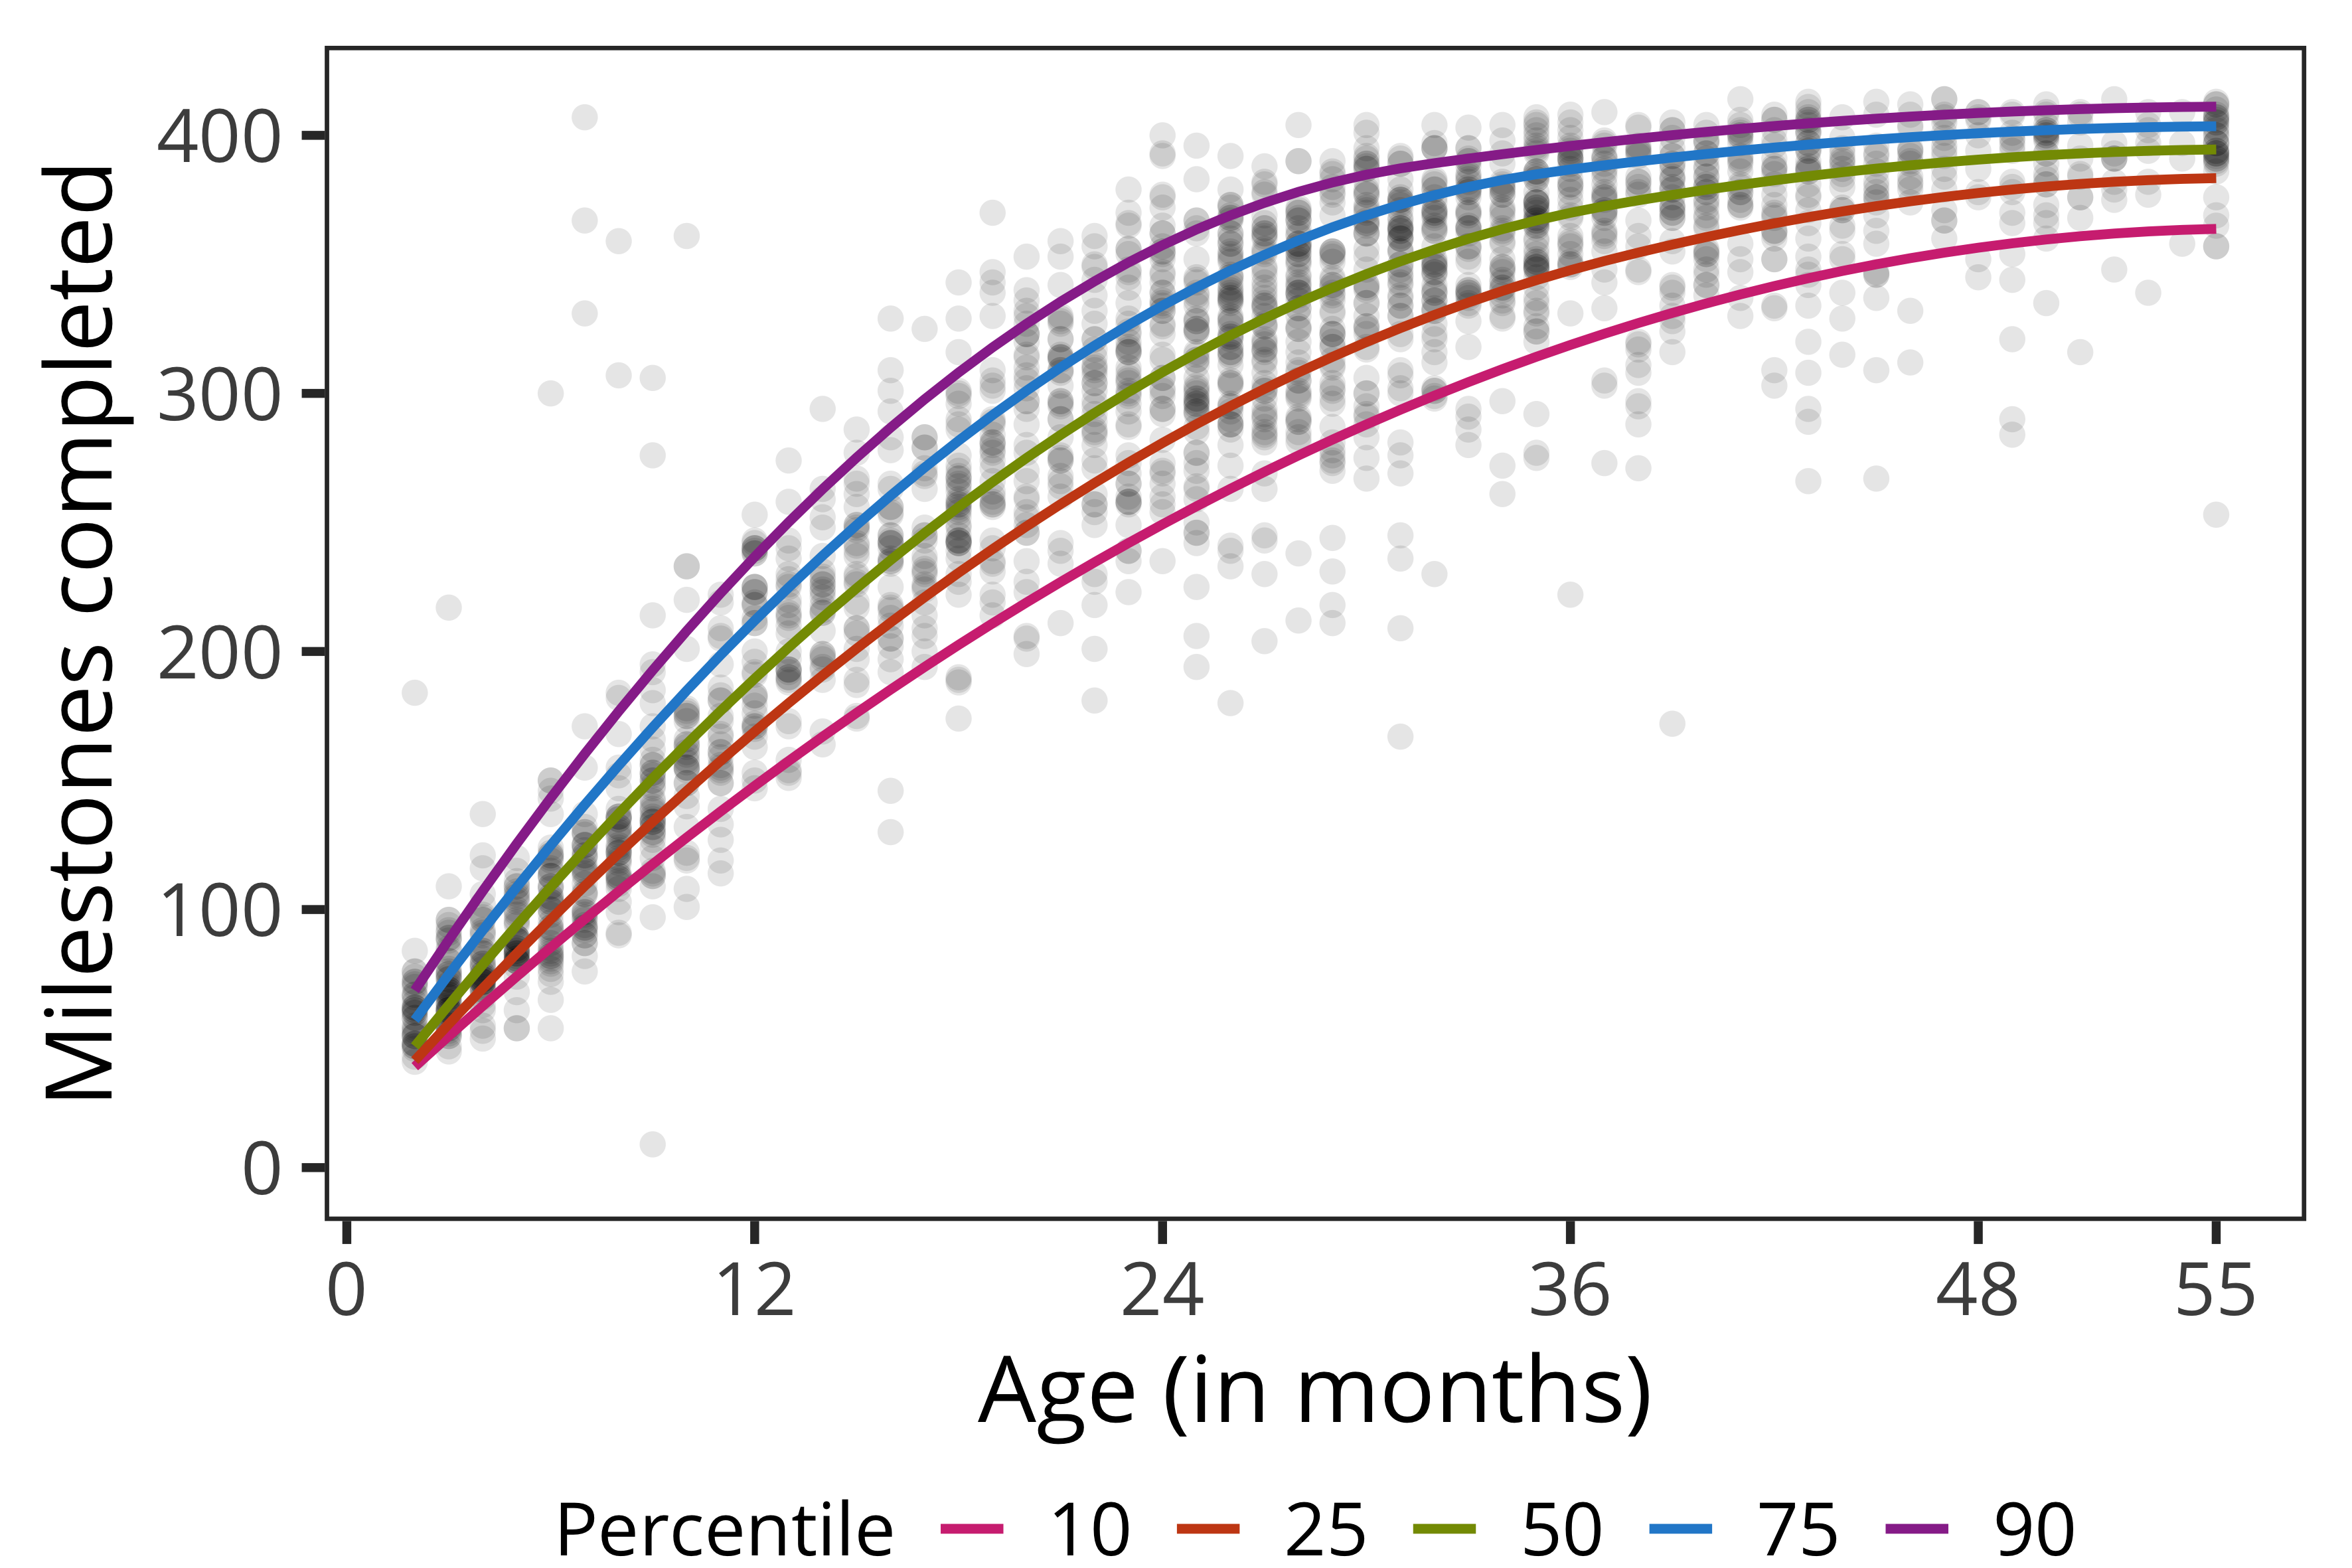
\includegraphics[width=1\columnwidth]{figures/01_achieve_by_age.png}
\caption{Number of the 414 milestones completed by age with percentile curves; data are from the survey reported in Study 1. Points represent individual children.}
\label{fig:partage}
\end{figure}

\hypertarget{item-response-models}{%
\subsection*{Item Response Models}\label{item-response-models}}
\addcontentsline{toc}{subsection}{Item Response Models}

% Educational testing and psychometrics uses a variety of item response
% theory models to design, analyze, and score many kinds of achievement
% tests. In brief, i
Item response models provide a robust framework for
assessing the structure of an instrument, the relative difficulty of
each item, and respondents' level of performance on the abilities or
latent factors measured by the instrument. Here, we use
two-parameter logistic (2PL) item response models to assess the
structure of children's development.

Let \(i = 1, \ldots, I\) represent the distinct children and
\(j = 1, \ldots, J\) the developmental milestones. The item response
data is stored in a matrix where element \(y_{ij}\) denotes if the
\(i\)th child has or has not achieved the \(j\)th developmental
milestone as reported by their parent/guardian. Each model represents
the \(i\)th child's development using \(m\) latent factors by
\(\boldsymbol{\theta}_{i}=(\theta_1, \dots, \theta_m)\). The \(j\)th
milestone's discriminations (i.e.~slopes)
\(\boldsymbol{a_j}=(a_1, \dots, a_m)\) capture the latent factor
loadings onto that milestone. We fit five 2PL models where a child's
development is represented by \(m = 1, \ m = 2, \ m = 3, \ m = 4\) and
\(m = 5\) latent factors (20). Hereafter, we, for example, refer to a
2PL model with \(m = 4\) latent factors as a 4F model. According to the
2PL model, the probability of child \(i\) having achieved  developmental
milestone \(j\) is \begin{equation}
P(y_{ij} = 1 | \boldsymbol{\theta_i}, \boldsymbol{a_j}, b_j) = \sigma(\boldsymbol{a}_{j}^{\top}\boldsymbol{\theta_i} + b_j)
\end{equation} where \(b_j\) is the milestone easiness (i.e.~intercept)
and \(\sigma(x) = \frac{e^x}{e^x + 1}\) is the standard logistic
function. 

By comparing models with varying numbers of factors, we learn about the
dimensionality of the construct measured by the instrument. If, for
example, models with numerous factors fit the data better than a 1F
model, then across-child comparisons are best made in a multidimensional
space.

We compare these item response models to a simple baseline
model that predicts achievement status based on milestone and age in
months. The baseline model always predicts the modal response for a particular milestone and age. For example, parents
report that 64\% of children age 16-months can identify animals by their sounds; the baseline model assumes that all 16-month-olds have reached this
milestone. This baseline aims to represent predictive performance in practical settings,
absent the use of item response models.

\hypertarget{study-1-the-structure-of-developmental-variation-across-individuals}{%
\section*{Study 1: The Structure of Developmental Variation Across
Individuals}\label{study-1-the-structure-of-developmental-variation-across-individuals}}
\addcontentsline{toc}{section}{Study 1: The Structure of Developmental
Variation Across Individuals}

We measure a model's fit to the data's structure based
on how well it predicts data previously unknown to the model (i.e.,
out-of-sample data) (21). In particular, we use cross-validation to compare
item response models with varying numbers of factors. We
partition the milestone responses into 8 folds. For each model, we
implement the following process. For each fold (the out-of-sample
fold), we estimate milestone and child development parameters using
milestone responses from the other 7 folds (the in-sample folds).
We use these parameters to make predictions for responses in the
out-of-sample fold. We aggregate performance from when each fold is
out-of-sample to calculate the overall out-of-sample accuracy of a
model. To estimate explained variance, we also extracted the proportion of variance explained by the model from a single fit of each model
to the full dataset (i.e., without cross-validation).

\hypertarget{developmental-variation-is-multidimensional}{%
\subsection*{Developmental Variation is
Multidimensional}\label{developmental-variation-is-multidimensional}}
\addcontentsline{toc}{subsection}{Developmental Variation is
Multidimensional}

Results from fitting the five different item response models are shown
in Table \ref{tab:study1results}. While the unidimensional model (1F:
88.8\% accuracy) fit better than the baseline (86.9\%), the
multidimensional models (2F to 5F) all fit the data better
(\textgreater{} 89.3\%). The 5F model provided 89.8\% out-of-sample
accuracy, and thus (of the models fit) provided the best predictive
performance. The 5F model explained less variance than the 4F model, however,
likely indicating that further increases in dimensionality would not yield better fit to data. 

Each of the models uncovered a consistent structure where linguistic milestones have
the greatest loadings on the 1st factor (i.e., linguistic milestone
discriminate well between children high and low on the 1st factor; Figure \ref{fig:discs}). For the 2F-5F models, physical milestones tend to have the greatest loadings
on the 2nd factor. Additional factors capture variation from fewer
milestones as seen by the majority of discriminations being relatively close to zero.

\begin{table}[!ht]
\caption{\label{tab:study1results}Model performance as measured by out-of-sample accuracy. Higher-dimensional models perform better.}
\centering
\fontsize{8}{10}\selectfont
\begin{tabular}[t]{lcc}
\toprule
Model & Out-of-sample Accuracy & Proportion of Variance\\
\midrule
5F & 89.8\% & 73.0\% \\
4F & 89.7\% & 74.5\% \\
3F & 89.5\% & 73.3\% \\
2F & 89.3\% & 66.1\% \\
1F & 88.8\% & 60.1\% \\
Baseline & 86.9\% & - \\
\bottomrule
\end{tabular}
\end{table}

\begin{figure*}
\centering
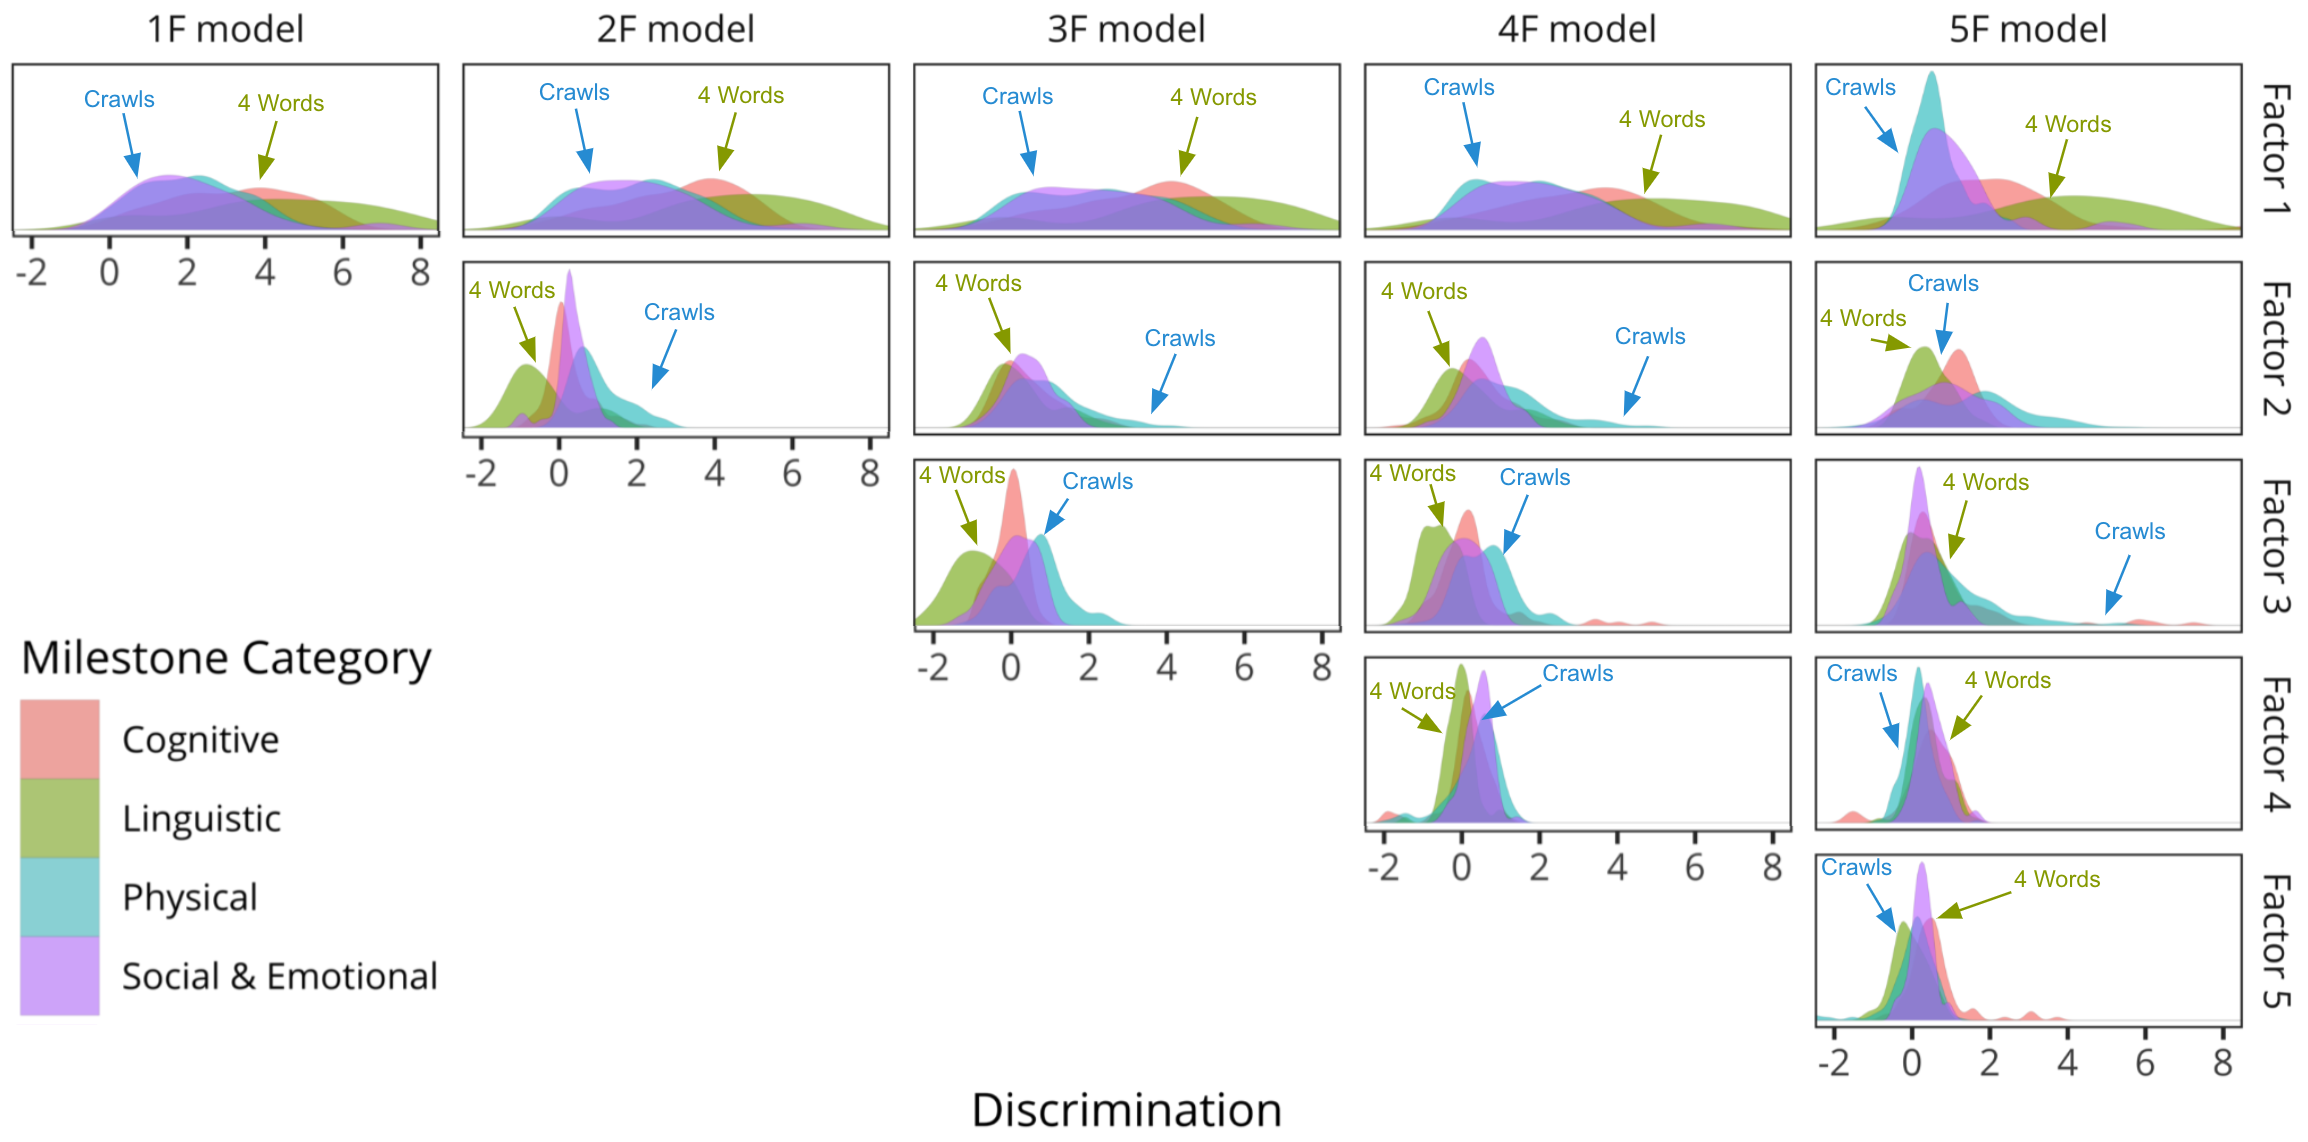
\includegraphics[width=1\columnwidth]{figures/models_new.png}
\caption{Distribution of discrimination parameters for the factors of the 1F, 2F, 3F, 4F, and 5F models. Columns of subplots show models, rows show factors, and distributions are the density of discrimination parameter estimates, colored by broad milestone categories. In each of the models, linguistic milestones load heavily on the 1st factor. Additional factors tend to be composed of other milestone categories—for example, physical milestones tend to load heavily on the 2nd factor. As expected, the typical discrimination decreases for later factors. Arrows track the location of two milestones, crawling (physical) and saying at least 4 words (linguistic), across each of the factors.}
\label{fig:discs}
\end{figure*}

\hypertarget{older-childrens-milestones-are-more-accurately-described-by-higher-dimensional-models}{%
\subsection*{Older Children's Milestones are More Accurately Described
by Higher-Dimensional
Models}\label{older-childrens-milestones-are-more-accurately-described-by-higher-dimensional-models}}
\addcontentsline{toc}{subsection}{Older Children's Milestones are More
Accurately Described by Higher-Dimensional Models}

The between-person version of the differentiation
hypothesis suggests that the abilities of older children have a
higher-dimensional structure. To examine the possibility of age-related differences in dimensionality we partitioned
the milestone data into roughly 1-year age groups: age 2 to 11 months,
12 to 23 months, 24 to 35 months, and 36 to 47 months and 48 to 55
months, with the upper two age groups consolidated together to
obtain similar sample size in each partition. We then calculated the gain
over the 1F model for each of the 2F to 5F models in each of the age-group partitions.
We calculated gain as the proportion of the distance between the 1F
model's performance and 100\% that the model achieves. For example, for
24 to 35-month-olds, the 5F model has 88.4\% accuracy as compared to the
1F model which has 87.2\% accuracy. The gain of the 5F model over the 1F
model, then, is \(\frac{88.4\% - 87.2\%}{100\% - 87.2\%} = 9.4\%\). The
top panel of Figure \ref{fig:study1} shows the gain of each
higher-dimensional model over the 1F model. The 5F model performs best
for each bin, and also performs particularly well for the older age
groups. The relative increase in gain for the 5F model (and other multi-dimensional models) at older ages is
consistent with the differentiation hypothesis.


\hypertarget{differences-between-old-children-are-better-described-by-higher-dimensional-models}{%
\subsection*{Differences Between Old Children Are Better Described by
Higher-Dimensional
Models}\label{differences-between-old-children-are-better-described-by-higher-dimensional-models}}
\addcontentsline{toc}{subsection}{Differences Between Old Children Are
Better Described by Higher-Dimensional Models}

Leveraging the sheer size of the data to push beyond evaluation of predictive performance of global models in different age groups, we also examined relative performance within each age-group partition separately. In particular, we conducted the 8-fold cross-validation procedure again within each partition of the data. The bottom panel of Figure \ref{fig:study1} shows the gain for
each of the higher dimensional models over the 1F model for each age
group fit separately. Using these age-partitioned models, we find similar but perhaps somewhat stronger evidence for the differentiation hypothesis: The gain of higher dimensional
models is modest for the youngest age group and substantially higher  for
older age groups.

\begin{figure}
\centering
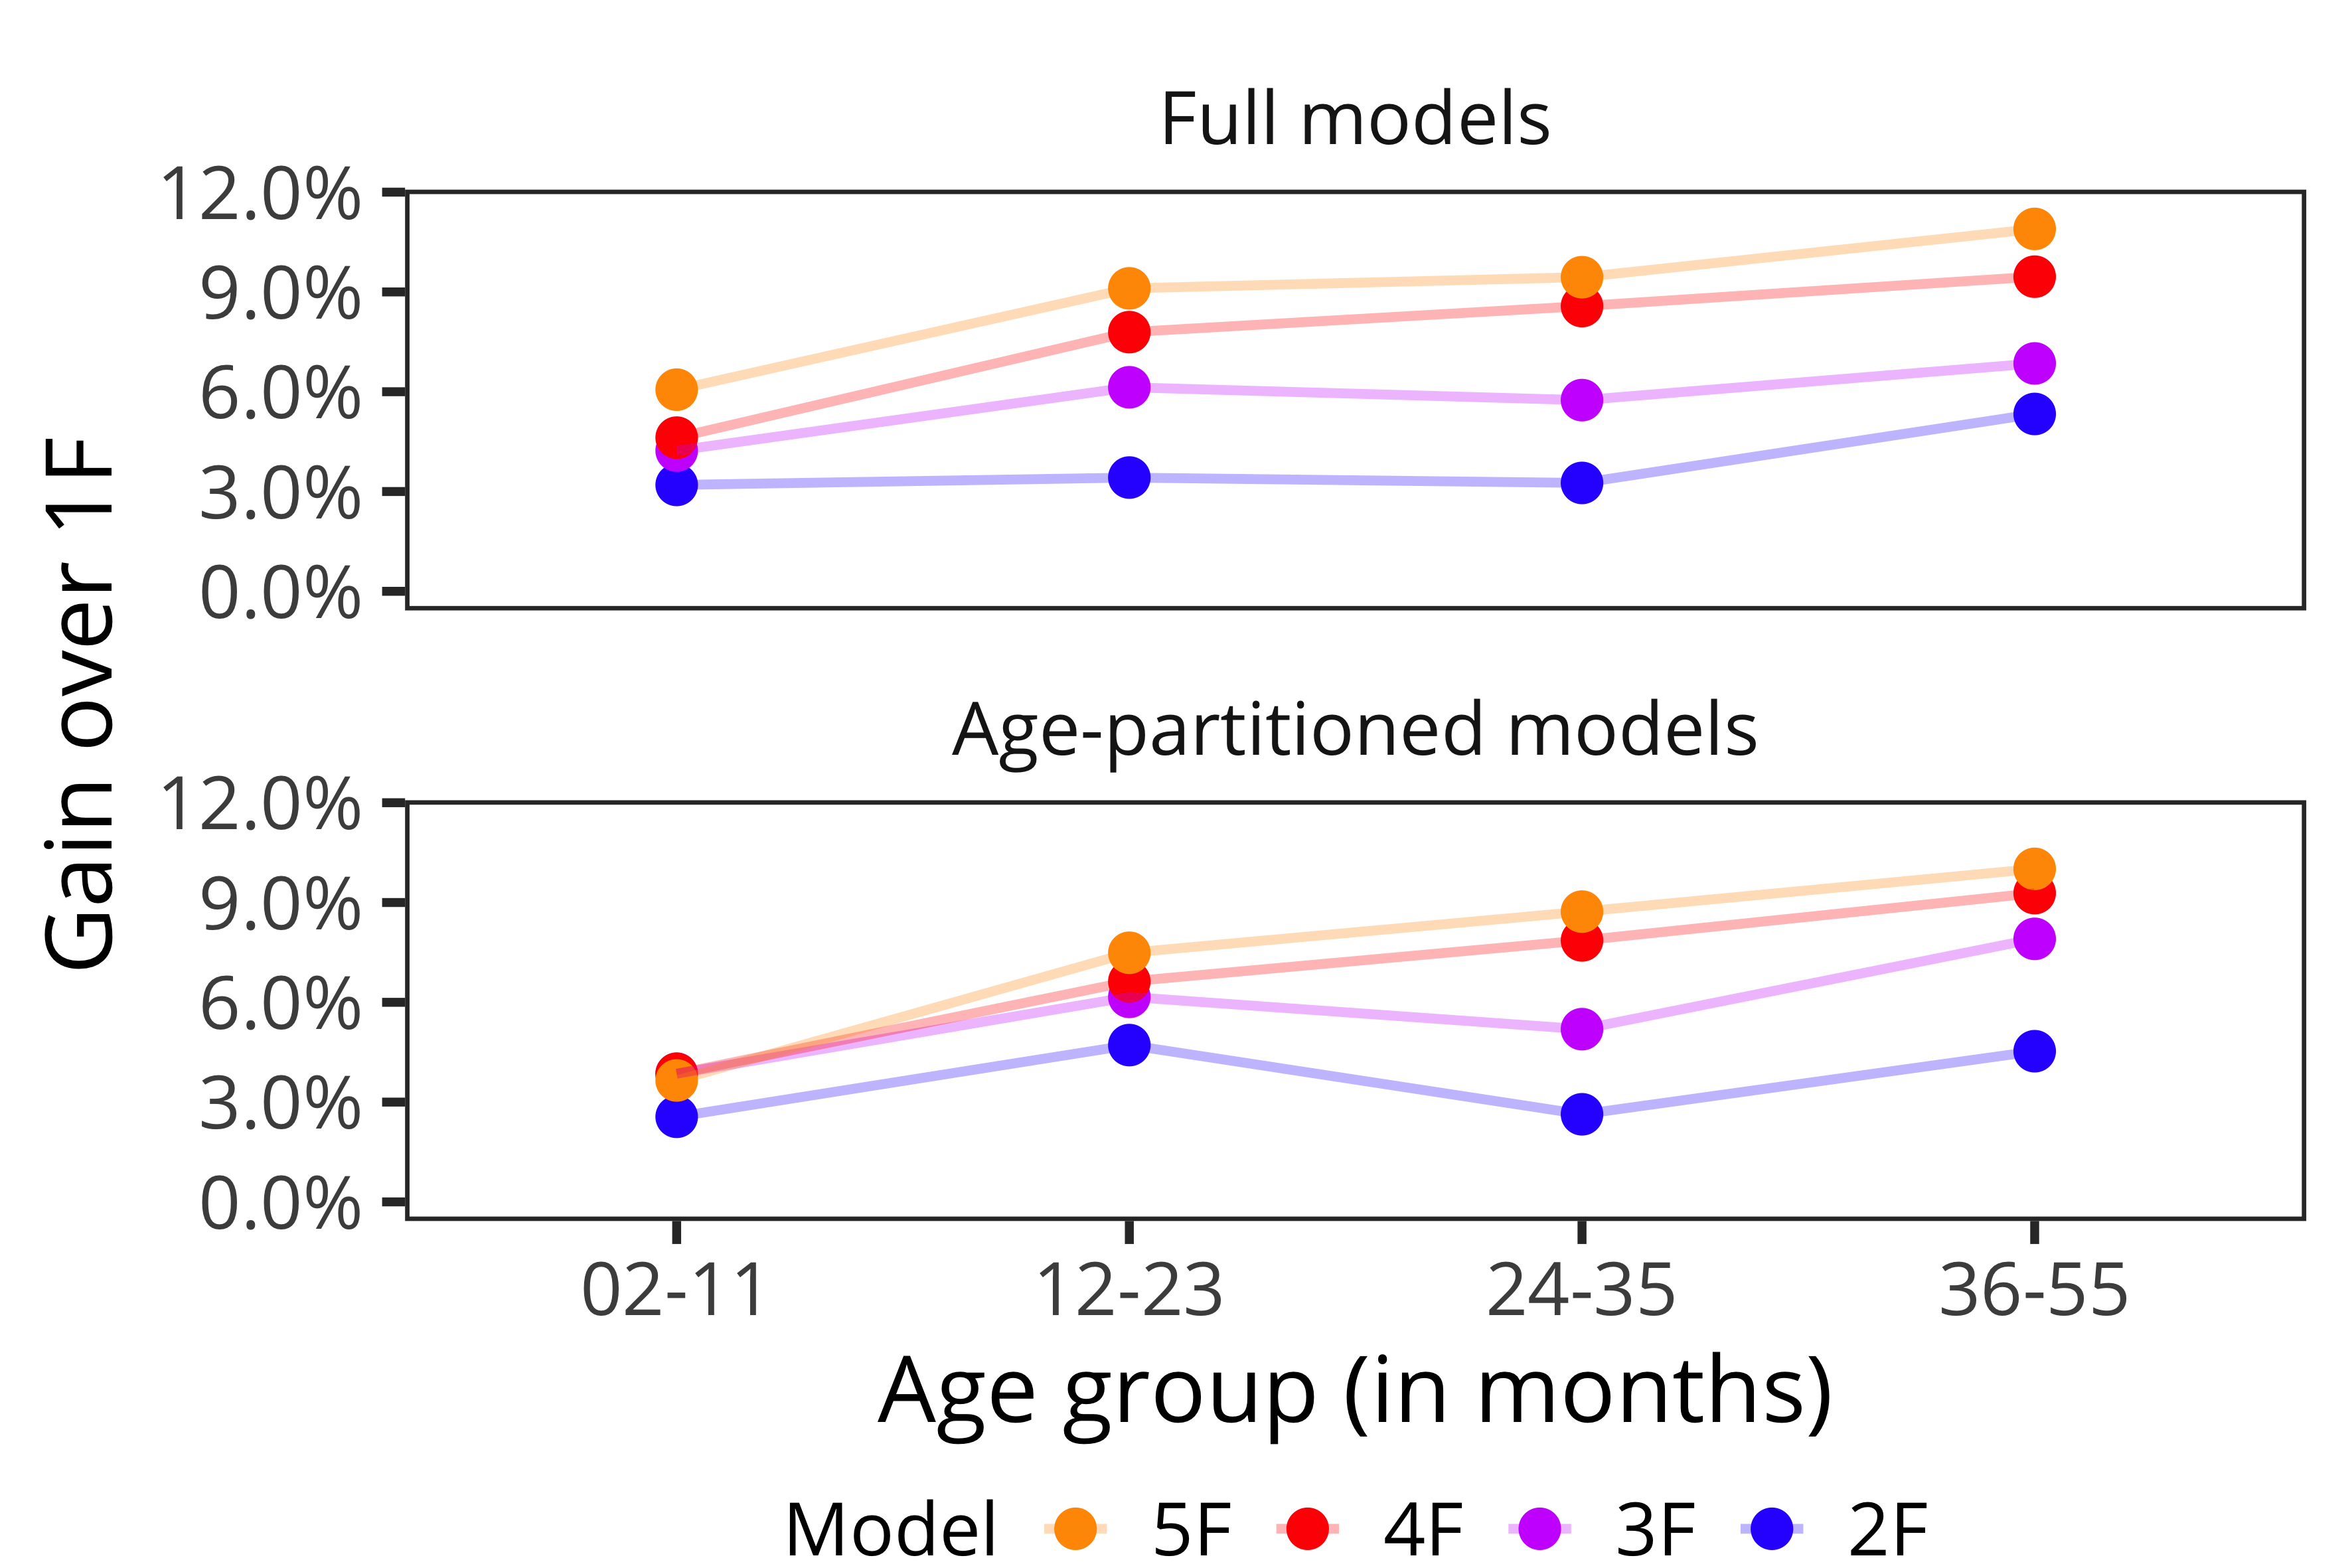
\includegraphics[width=1\columnwidth]{figures/study1.png}
\caption{Gain of higher-dimensional models over 1F model. Gain is defined as the proportion of the distance between the 1F model’s performance and 100\% that the model achieves. The top panel shows that when each model is fit to the full dataset, higher-dimensional models perform particularly well for older age groups. The bottom panel shows that when each model is fit separately to each age group, higher-dimensional models perform particularly well for older age groups.}
\label{fig:study1}
\end{figure}

\hypertarget{study-2-the-dimensionality-of-within-child-variability-increases-across-development}{%
\section*{Study 2: The Dimensionality of Within-Child Variability
Increases Across
Development}\label{study-2-the-dimensionality-of-within-child-variability-increases-across-development}}
\addcontentsline{toc}{section}{Study 2: The Dimensionality of
Within-Child Variability Increases Across Development}

Drawing conclusions about within-child processes using between-child
data risks committing a version of the ecological fallacy. The
ecological fallacy typically cautions against making individual-level
claims from group-level data (22). In the case of the differentiation
hypothesis, the ``group'' is the child and the ``individual'' is each of
the timepoints that the child is measured at. Patterns across children
are not necessarily indicative of patterns across individual childrens'
timepoints. Therefore, the best assessment of the differentiation
hypothesis requires longitudinal data.

We leverage the use of Kinedu, Inc.'s application as our source of such
longitudinal data. As part of using the app, parents are asked to
respond to 20-50 milestones about their child every few months. As with
many mobile apps, usage is non-uniform, such that many users use the app
once or only occasionally, while a smaller number used it frequently. We focus here on the most frequent users of the app, as their relatively dense data provide the best opportunity to test hypotheses about within-child change. We
selected data from children with at least 6 timepoints, where a
timepoint contains at least 5 responses to each of the 4 milestone
categories. We also focus here on children between 2 and 18 months old
because parents typically use the app when their child is in this age
range and so there were few children with dense data in older age ranges.

A previous test of the de-differentiation hypothesis using longitudinal data
examined deviations from individual developmental pathways to identify how these deviations related to one another (10). We adapt this
method, which was developed for continuous outcomes, to factor scores
estimated from binary outcomes. In brief, the goal of this method is to ask whether local deviations from the child's own developmental trajectory are related to one another ("coupling"). For example, if a child surges ahead on motor milestones in a particular month, will they also surge ahead on linguistic milestones? 

Computing coupling of this type involves five distinct steps (Figure
\ref{fig:study2} visualizes the first four). The first step was to develop an
appropriate measurement model. Because the survey data is complete and
likely to be higher quality, we chose to use the survey data to develop
this model. To ensure that the model was well-calibrated for the app
data, we filtered to children 24 months of age or younger and removed a
small number of children with an unexpected number of milestones
complete for their age (e.g., a 9-month-old with more than 350
milestones complete). A 2F model offers good fit and an interpretable
factor structure for this population. The 1st and 2nd factors capture 35\% and
20\% of the survey data variance, respectively (an additional factor
would explain only 5\% more variance). These factors appear to load more heavily on physical milestones vs. linguistic milestones, respectively. Although models with more factors
show the same differentiation effect described below (see SI), the
finding is easiest to conceptualize in a two-factor space.
 
% The logic of our method is based on
% viations from a child's developmental pathway. 

The second step was to estimate factor scores for each
child-timepoint in the app data according to the parsimonious 2F model
fit to the survey data. As expected, these factor scores are highly
correlated with age. In the third step, we separately estimated a
quadratic developmental pathway for each child. In the fourth step, we
calculate the deviation from the child's developmental pathway for each
timepoint.

\begin{figure*}
\centering
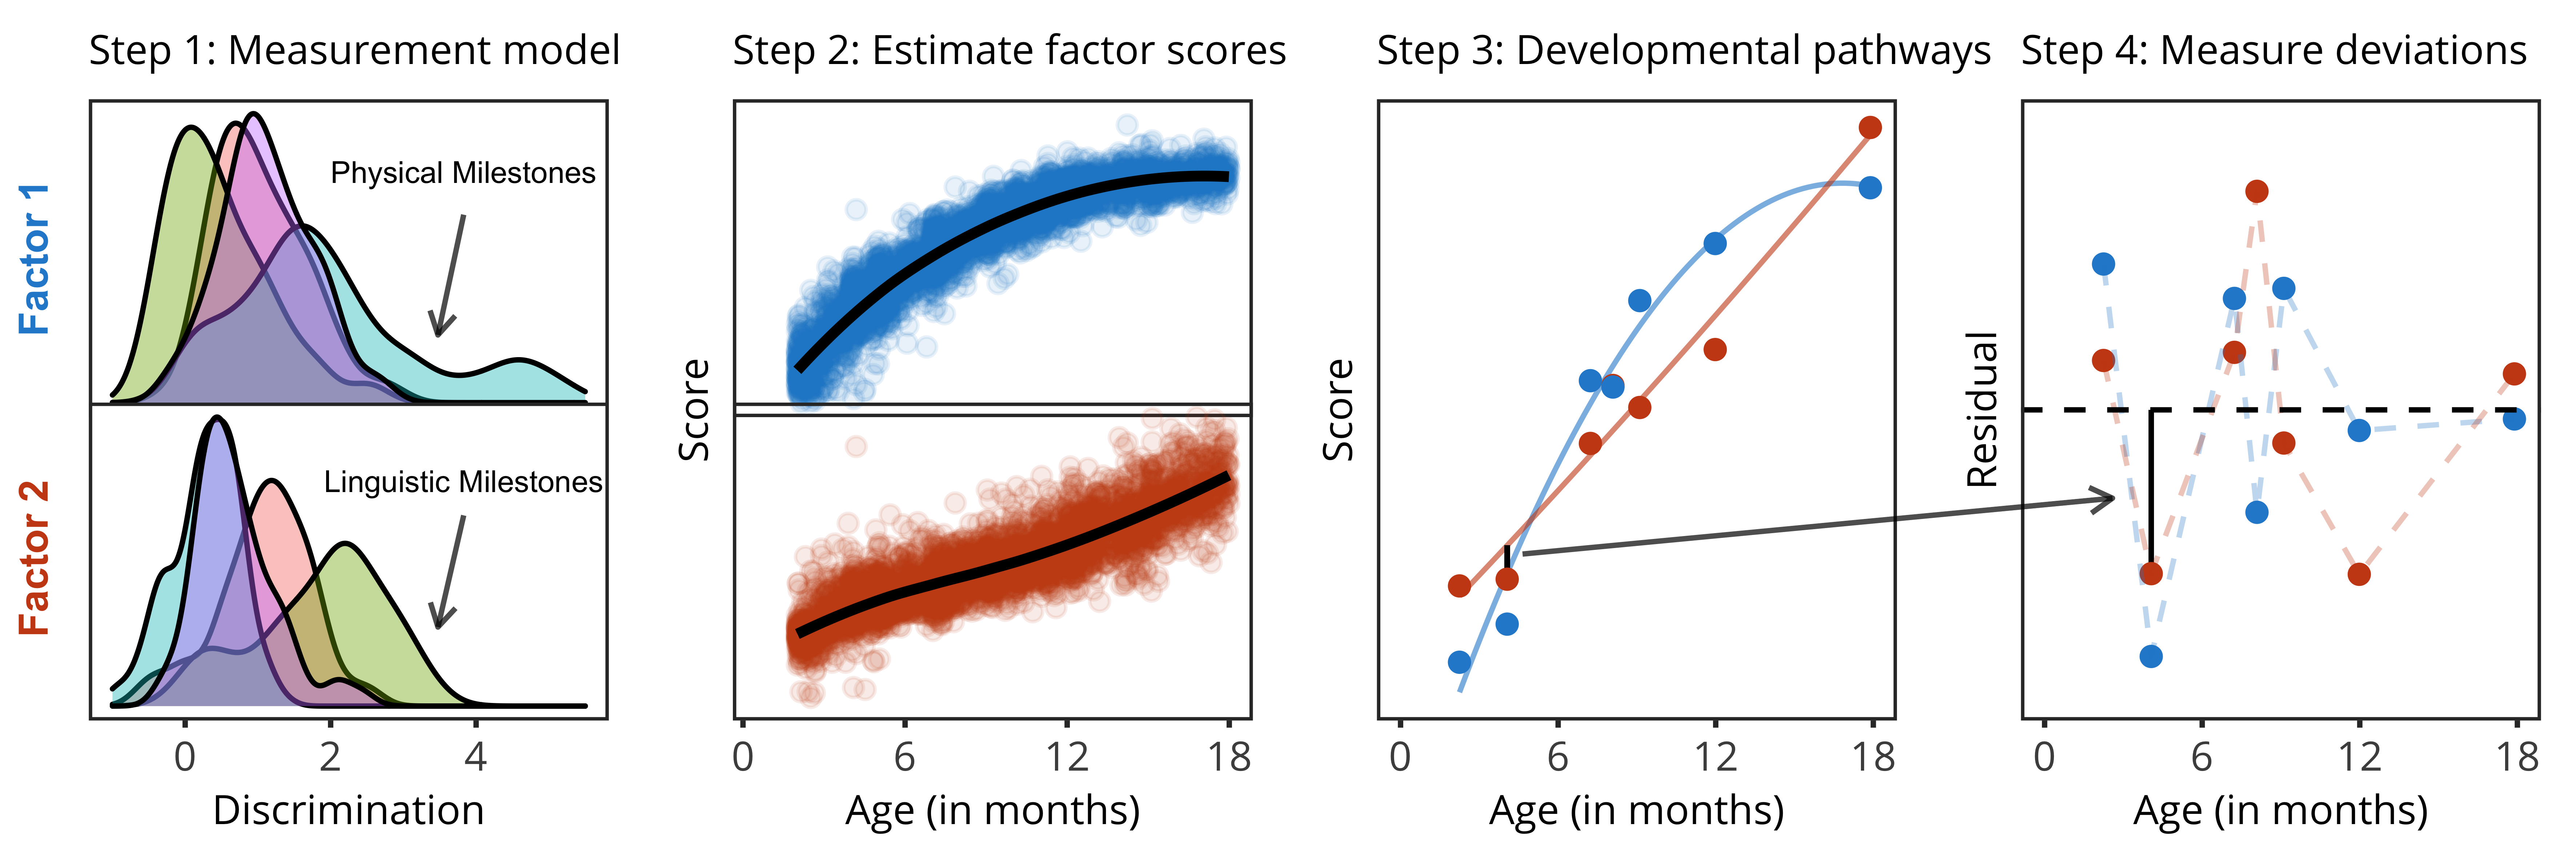
\includegraphics[width=1\columnwidth]{figures/bigfigure.png}
\caption{Each panel corresponds to a step from Study 2. In the first step, we used the survey data to develop a measurement model. The first factor is mainly physical and the second factor is mainly linguistic. In the second step, we used the measurement model to estimate factor scores for each child-timepoint in the app data. As expected, both factors are highly associated with age. In the third step, we modeled longer-term developmental trends separately for each child. Here, we illustrate this step by showing the trends for a single child. In the fourth step, we extract the deviations (i.e., residuals) from the developmental trends. Here, we show the deviations (i.e., residuals) for that same child. These deviations allow us to examine age-related differences
in within-person coupling of factor scores.}
\label{fig:study2}
\end{figure*}

The fifth and final step was to fit a mixed-effects model to estimate
coupling across the age span for all children. The model predicts the deviation for one factors using the other factor's deviation (and interactions with age), while controlling for differences between individual children using random effects (following 10). Larger coefficients on factor deviation indicate greater coupling, such that, for example, if at a particular time point the child increases on factor 1 they are more likely to increase on factor 2. 

In developing our method, we used an exploratory sample of 600 children (4,734 timepoints, $M$=7.9 timepoints/child). We then replicated the procedure using two additional samples of 600 children (we leave some data unanalyzed for future exploration). In all
three samples, we find strong evidence for the differentiation
hypothesis. For example, a 1-unit deviation from factor 2's
developmental pathway is associated with at least a 0.75-unit deviation
in the same direction from factor 1's developmental path at 2 months
old. And, this association decreases to less than a 0.15-unit deviation
for children older than 12 months old. We find similar results when
inverting the factors and considering the association between deviations
from factor 1's developmental pathway on deviations from factor 2's
developmental path. These results are depicted in Figure
\ref{fig:study2results}. 

In sum, this finding gives strong evidence that, within individual children, local deviations from the child's own developmental growth trajectory begin quite coupled but appear to decouple by around 18 months. Put another way, when a young baby grows especially quickly or slowly they tend to do so on all relevant dimensions (at least within our milestone set). In contrast, a toddler's language can surge forward (or hang back) without coordinated changes in motor development. Thus, we find evidence for the differentiation hypothesis within individual children.

\begin{figure}
\centering
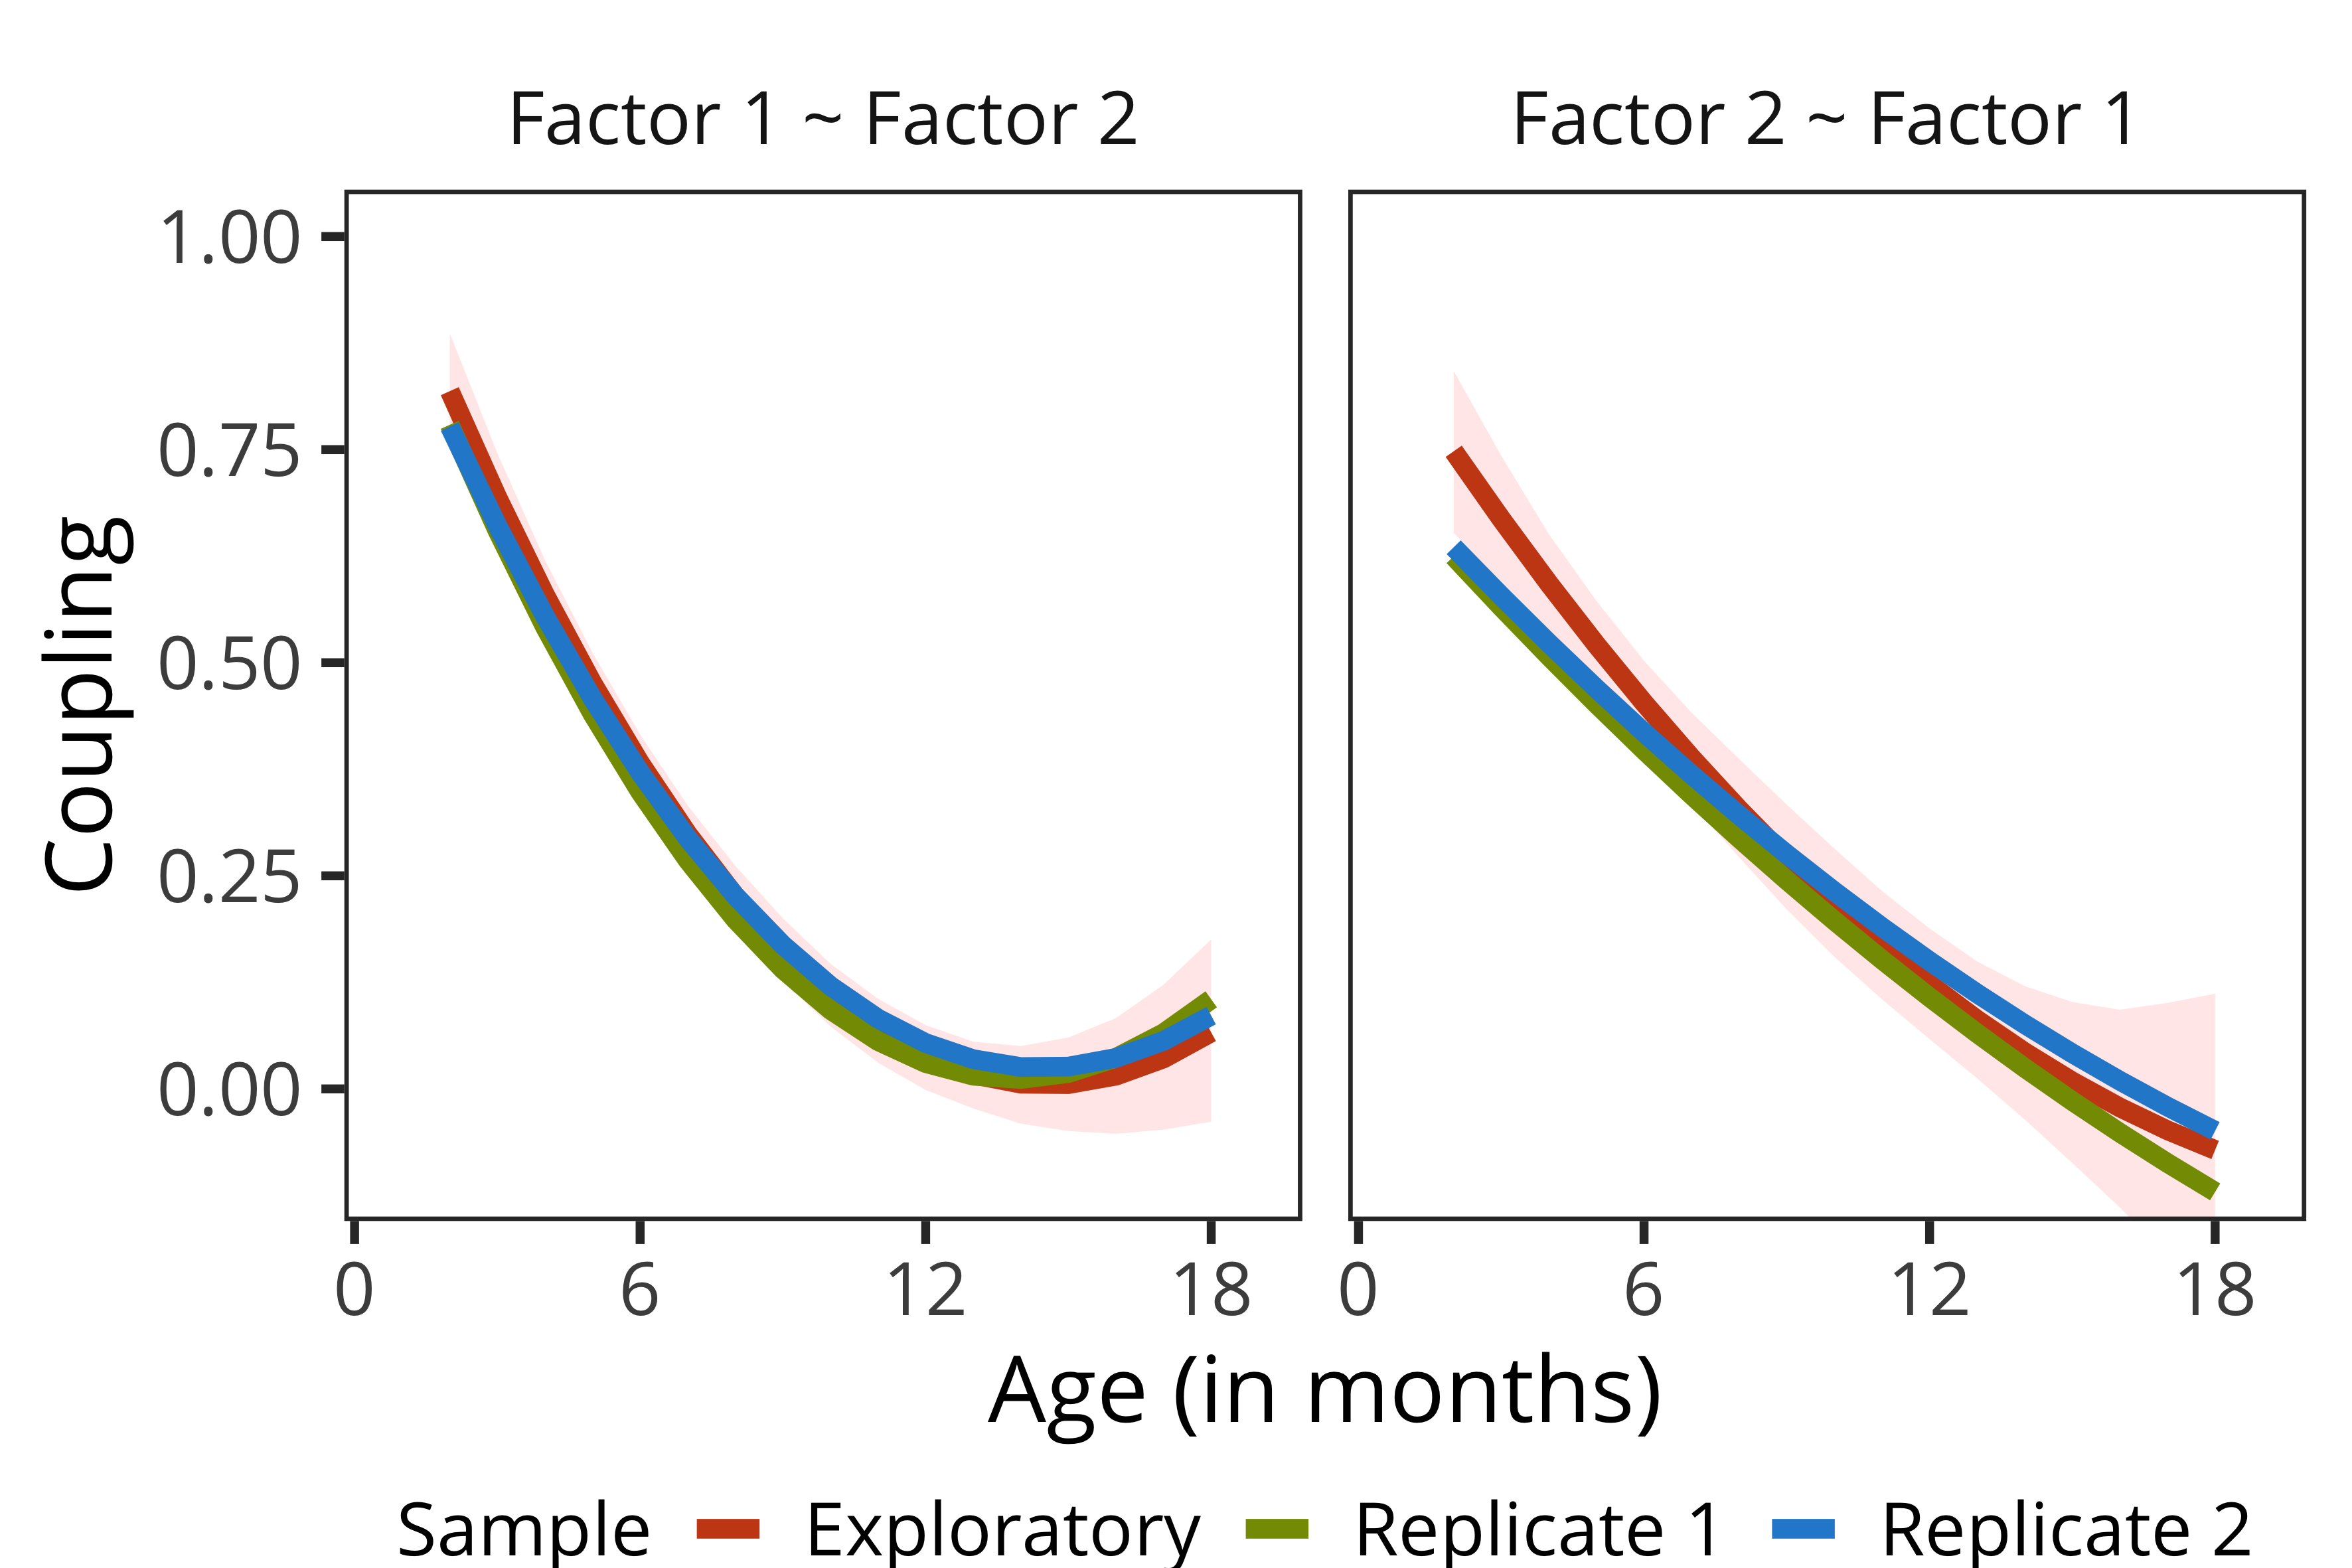
\includegraphics[width=1\columnwidth]{figures/study2results.png}
\caption{Coupling parameters from 2 to 18 months old. Association between 1-unit deviation from the developmental pathway for one factor with deviation from the other factor’s developmental path. Left panel shows factor 1 as the dependent variable and factor 2 as the independent variable. Right panel is the inverse. As the differentiation hypothesis suggests, we find decreasing coupling over the age span. Red shading is 95\% confidence interval for exploratory sample as calculated by 1000 bootstrapped simulations.}
\label{fig:study2results}
\end{figure}

\hypertarget{discussion}{%
\section*{General Discussion}\label{discussion}}
\addcontentsline{toc}{section}{General Discussion}

Is child development a single unified process or a host of different
processes? Stage theories assume synchronization in developmental
changes across distinct domains like language, social-emotional
development, and cognition (1). In contrast, more modern modular theories
tend to assume that particular aspects of development proceed ``on their
own schedule'' (3,23). Here, inspired by psychometric studies of
age-related changes in cognition, we explored this issue through the lens of individual variation. Our premise was that
understanding the nature of variation in developmental milestones could help shed
light on whether children's developmental change covaries across domains
within a single factor and whether developmental variation splits into multiple factors as children grow older.

With the emergence of data science techniques, our use of newly
available data is a specific instance of a general pattern: Larger data
enables more precise measurements, which can be used to test and refine theories.
Although theorists have speculated about developmental differentiation,
to our knowledge the differentiation hypothesis had not previously been tested using large-scale
data. Our contributions came from leveraging data made newly available
due to parents' use of a mobile app. Parents, who were looking to understand and
support their child's development, answered hundreds of binary milestone
questions about their child. As a result, we were able to explore and
test the differentiation hypothesis in early childhood by fitting a
variety of psychometric models to this data.

% What are the developmental factors that these models identified? 
We modeled the structure of age-related variation between children and identified data-driven dimensions in this variation. These appeared to map to some extent onto classic domains of development, for example by loading more heavily on motor or language milestones.
It is important to remember, however, that by nature of our analyses, our results describe differences rather than commonalities between individuals. Because we leverage individual variability, our models are not designed to detect the operation of mechanisms that are consistent across individuals. Despite the variation we observed and quantified,
many common mechanisms (from statistical learning to motor skill learning) likely support developmental change across all individuals. The individual differences in milestones that we observe then might simply be differences in  learning rates across individuals.

Our study has several limitations that should inform future work. First,
we relied on parent report, which can have significant biases and
limitations, especially in its precision regarding capacities that are
difficult to observe (e.g., cognitive abilities: 16, 24). Second, our
data come from very specific populations (Study 1: middle- and
upper-class Mexican parents whose children were in group care; Study 2:
an unknown but largely Brazil, US, and Mexico-based group of users of a developmental mobile application) and hence
caution is warranted in generalizing to specific populations. Third, our results are with regard to child development
as defined by the Kinedu app milestone set. These milestones provide a global picture of observable developmental changes, but they do not necessarily carve development at its joints. Further, the factor discovery methods we use reflect the statistical structure of the observed data rather than the structure of any latent variables internal to the child (25--27).

In the end, our goal is a first step in the direction of leveraging
large datasets to better understand child development. Our approach was
to combine multiple data sources and develop novel methods which
together allowed us to explore theories of child development. In doing
so, we found multidimensionality in the variation between children and support for the
development differentiation hypothesis both across and within children. Our hope is
that this work encourages others to continue to advance developmental
theory by taking advantage of opportunities provided by new, 
larger data sources.

\hypertarget{mat}{%
\section{Materials and Methods}\label{mat}}
All data were provided by Kinedu, Inc. A pre-registration, code, and data are publicly available at https://osf.io/5426p/. We deviated from the pre-registration for two reasons. First, we had not planned to use longitudinal data but came to appreciate the importance of these data for examination of differentiation as a within-person phenomenon. Second,
we had failed to appreciate the degree to which lack of milestone
overlap across ages (i.e., planned missingness for older children to
younger milestones and vice versa) jeopardize making valid cross-age
comparisons. In our Supplemental Information, we report on an additional dataset that we preregistered the intent to analyze, but eventually deemed unsuitable for these reasons. 

\subsection*{Survey Data}

The survey data used in Study 1 was collected by Kinedu, Inc.~during the
development of their mobile application. The surveys were completed by
middle- and upper-class Mexican parents whose children were in group
care. The raw survey data contains complete (i.e., no missingness)
responses to all 414 milestones for 2,023 children. We filtered out
children younger than 2 months old due to concerns about data quality
(e.g., 40\% of 0- and 1-month-olds had surprisingly achieved at least 80
milestones). The analysis data for our examination of dimensionality
(Study 1) included data on whether or not 1,946 children age 2 to 55
months had achieved 414 cognitive, linguistic, physical and
social-emotional milestones.

\subsection*{App Data}

The app data focused on in Study 2 was collected by Kinedu, Inc.~during
normal operations of their development mobile application. In
particular, the app asks parents to report on age-appropriate milestones
for their child every few months. We considered data collected between
the beginning of the current 414 milestones (12/01/2017) and the start
of data analysis for this part of the project (12/16/2020). Our goal was
to create a longitudinal dataset. We created ``timepoints'' based on
milestones responses that were collected within a 5-day window for each
child. We subset down to timepoints where a significant number of
milestones were responded to---specifically, we required at least 5
responses to each of the 4 milestone categories for a total of at least
20 responses. To target the app's typical users, we considered only
timepoints when the child was at least 2 months old and less than 18
months old. We did so both to mitigate any floor or ceiling effects and
to reduce any potential selection bias that might result from parents
who elect to use the app when their child is older than was typical.
Finally, so as to have sufficiently longitudinal data for each child, we
considered only children with at least 6 such timepoints. The result of
these pre-processing steps was the ``app data'' containing 21,861 unique
children and 177,934 total timepoints. We used only 1,800 of these
children in the form of three 600 child samples. Each sample was drawn
randomly. The first sample (the exploratory sample) was used while
developing methods. The second and third samples (the replication
samples) were used to test the validity of results from the exploratory
sample.

\subsection*{Study 1: Dimensionality of Developmental Milestones in Early Childhood (Cross-validation of Item Response Models)}

To examine the structure and dimensionality of children's achievement of
developmental milestones, we compared the relative fit of item response
models with between 1 and 5 factors. Model comparison in IRT typically
uses information criterion such as AIC and BIC (28). However, these
methods are not guaranteed to work with modest sample sizes or when the
models are misspecified (29). Instead, we implemented a version of
cross-validation for item response models with varying numbers of
factors (30). The steps of our cross-validation procedure are as
follows. We began by partitioning the data into 8 folds. We stratified
randomization by child so that each fold contained approximately
one-eighth of each child's milestone responses. In other words, each
child was split into 8 ``sub-children'' and each fold contained exactly
one of these sub-children. We refer to the fold hidden from the data as
out-of-sample and the other 7 folds as in-sample. Holding each of the 8
folds out one at a time, we then conduct the following steps for each
model.

We first fit the model to the in-sample data. According to an
m-dimensional 2PL model, the probability of a child having achieved a
developmental milestone is \begin{equation}
P(y_{ij} = 1 | \boldsymbol{\theta_i}, \boldsymbol{a_j}, b_j) = \sigma(\boldsymbol{a}_{j}^{\top}\boldsymbol{\theta_i} + b_j)
\end{equation} where the \(j\)th milestone's discriminations
(i.e.~slopes) \(\boldsymbol{a_j} = (a_1 ,..., a_m)\) capture the latent
factor loadings onto that milestone; \(b_j\) is the milestone easiness
(i.e.~intercept); and \(\sigma(x) = \frac{e^x}{e^x + 1}\) is the
standard logistic function. We stabilize the model by using a Normal(0,
3) prior on all \(b_j\) values. We do not use a prior on so as to not
interfere with interpretations of dimensionality. As is common for item
response models, we used marginal maximum likelihood estimation (MMLE),
which estimates milestone parameters but not child parameters (31).
Higher dimensional models require slightly different estimation methods
so the full latent factor space is adequately considered: For models
with 3, 4, or 5 factors, we used quasi-Monte Carlo EM estimation (32);
for models with 1 or 2 factors we used the standard EM algorithm (33).
To allow for correlations in the factor structure, we estimated
milestone parameters under an oblimin rotation (34).

Second, we estimated factor scores for each child using the in-sample
data. We estimated factor scores using expected a posterior (EAP) with a
m-dimensional normal prior as calculated by Gauss-Hermite quadrature
(35). Third, we use the milestone parameters and factor scores estimated
using the in-sample data to predict the probability of each
out-of-sample milestone response.

Going through these steps for each fold resulted in a predicted
probability for each milestone response. We evaluated each model's fit
by simply considering these predictions' accuracy (correct if the
predicted probability was greater than 50\% and the milestone was
achieved or if the predicted probability was less than 50\% and the
milestone was not achieved). We compared these models to a simple
baseline model that makes predictions based on a child's age (in months)
and the milestone. For example, parents reported that 64\% of
16-month-olds can identify animals by their sounds, so the baseline
model predicts that all 16-month-olds have reached this milestone (when
fewer than 50\% of children at that age had not achieved the milestone,
the baseline model predicts that none of the children at that age in
months have achieved the milestone).

We examined the relationship between age and dimensionality using two
techniques. Both techniques involve measuring the relative gain of a
higher dimensional model relative to a 1F model. Letting
\(\text{acc}_\text{model}\) represent the out-of-sample accuracy from a
higher-dimensional model and \(\text{acc}_\text{1F}\) represent the
out-of-sample accuracy from a 1F model, we calculated gain as
\(\dfrac{\text{acc}_\text{model} - \text{acc}_\text{1F}}{1 - \text{acc}_\text{1F}}\).
Intuitively, gain can be thought of as the higher dimensional model's
percent of possible improvement in accuracy over the 1F model. Our first
technique was break down each model's performance by age group so that
we could calculate the gain by age group. This involved estimating 40
models (\(5 \text{ models} \cdot 8 \text{ folds}\)). If the structure of
developmental variation changes with age, then it may be suboptimal to
estimate models based on all children. Accordingly, our second technique
was to estimate each model separately for each of the age groups. This
involved estimating 200 models
(\(5 \text{ models} \cdot 8 \text{ folds} \cdot 5 \text{ age groups}\)).
We then calculated the gain for each model in each age group. For some
age groups, nearly all (or no) children have accomplished some of the
milestones. To prevent these milestones from destabilizing model
estimation, we filtered out milestones from an age group's data when
more than 97.5\% or fewer than 2.5\% of children had achieved the
milestone. Figure \ref{fig:study1} shows results from both techniques,
with the top panel corresponding to the first and the bottom panel
corresponding to the second.

\subsection*{Study 2: Testing the Differentiation Hypothesis Using Longitudinal Item Response Data}

The differentiation hypothesis suggests that the structure of children's
abilities expands with age. In Study 2, we use the longitudinal app data
to test this hypothesis. To do so, we adapt methods developed in
examination of dedifferentiation of cognitive abilities in old age (10)
to analysis of factor scores obtained from multidimensional item
response models of the milestone data obtained on up to 21 occasions as
children moved through early childhood. As detailed below, we use
multilevel model models of change to examine if and how age moderates
the extent of within-person coupling in the occasion-to-occasion changes
in factors underlying milestone achievement (estimated using item
response models), after controlling for individuals' general
developmental gains. Our expectation is that, separate from the
long-term developmental trends, within-person variations on 2 underlying
ability factors will be tightly coupled (i.e., dedifferentiated) at
earlier ages and that the extent of coupling will decrease towards zero
as children get older and the underlying factors differentiate. Analysis
proceeded in five steps: (1) develop a measurement model, (2) estimate
factor scores, (3) model longer-term developmental trends, (4) extract
deviations from longer-term developmental trends, and (5) examine
age-related differences in within-person coupling of factor scores. The
first four steps are shown in Figure \ref{fig:study2}. The fifth step is
shown in Figure \ref{fig:study2results}.

\hypertarget{step-1-develop-a-measurement-model}{%
\subsubsection*{Step 1: Develop a Measurement
Model}\label{step-1-develop-a-measurement-model}}
\addcontentsline{toc}{subsubsection}{Step 1: Develop a Measurement
Model}

Our first analytic task was to obtain measurement invariant factor
scores from the longitudinal milestone achievement data. Taking a
relatively conservative approach, we use a filtered version of the
survey data. We did so because (a) the app data skews younger than the
survey data and (b) the survey data started to show ceiling effects at
24 months old (see Figure \ref{fig:partage}). In particular, we filter
the survey data to children between 1 and 24 months old (931 of the
2,023 children). We also filter outlier children by considering only
children with more than \(15 + 8 \cdot \text{age in months}\) and less
than \(100 + 14 \cdot \text{age in months}\) milestones achieved (909
out of 931 children). We measure age in months where a month is 30.3
days. We used a 2F model because our goal was to understand the
relationship between main factors (a 2F model explained 55\% of the
variance; a 3F model explained 60\% of the variance). We estimated
milestone parameters by using MMLE to fit this 2F model, which specifies
the probability of child \(i\) having accomplished milestone \(j\) as
\begin{equation}
P(y_{ij} = 1) = \sigma(a_{j1}\theta_{i1} + a_{j2}\theta_{i2} + b_j)
\end{equation} where \(a_{j1}\) and \(a_{j2}\) are milestone \(j\)'s
slope with respect to factor 1 and 2, respectively; \(\theta_{i1}\) and
\(\theta_{i2}\) are child 's factor 1 and factor 2 scores, respectively;
and \(b_j\) is milestone \(j\)'s easiness. As is common when fitting a
multidimensional item response model with a limited sample size, we used
priors to stabilize the model. In particular, we used a Normal(0, 3)
prior on \(b_j\) and a Lognormal(0, 0.5) prior on \(a_{j1}\) and
\(a_{j2}\) values. Given that the factors were high correlated, an
oblique rotation was required. Accordingly, we estimated milestone
parameters under an oblimin rotation (34).

\hypertarget{step-2-estimate-factor-scores}{%
\subsubsection*{Step 2: Estimate Factor
Scores}\label{step-2-estimate-factor-scores}}
\addcontentsline{toc}{subsubsection}{Step 2: Estimate Factor Scores}

The model parameters were tabulated and used to estimate factor scores
using EAP with a 2-dimensional normal prior as calculated by
Gauss-Hermite quadrature (35), for each of the children on each occasion
in the longitudinal app data. Importantly, these factor scores capture
within-person changes in two measurement invariant ability factors
underlying children's achievement of cognitive, linguistic, physical and
social-emotional milestones across early childhood, age 2 to 55 months.

\hypertarget{step-3-model-longer-term-developmental-trends-and-step-4-extract-deviations}{%
\subsubsection*{Step 3: Model Longer-term Developmental Trends and Step
4: Extract
Deviations}\label{step-3-model-longer-term-developmental-trends-and-step-4-extract-deviations}}
\addcontentsline{toc}{subsubsection}{Step 3: Model Longer-term
Developmental Trends and Step 4: Extract Deviations}

Having obtained estimated factor scores for each factor on each occasion
for each child, we proceeded to model the systematic age-related changes
in each factors. Separately for each child, the longitudinal factor
scores for the first factor were modeled as \begin{equation}
\theta_{1ti} = B_{10i} + B_{11i}(age_{ti}) + B_{12i}(age^2_{ti}) + e\theta_{1ti}
\end{equation} where the estimated factor score for child \(i\) on
occasion \(t\), was modeled as a trajectory defined by a person-specific
intercept \(B_{10i}\), a person-specific linear slope, \(B_{11i}\), a
person-specific quadratic slope, \(B_{12i}\). Deviations from the age
trajectory, then are captured by the person- and occasion-specific
residuals, \(e\theta_{1ti}\). In parallel, the longitudinal factor
scores for the second factor were modeled as \begin{equation}
\theta_{2ti} = B_{20i} + B_{21i}(age_{ti}) + B_{22i}(age^2_{ti}) + e\theta_{1ti}
\end{equation} where the estimated factor score for child \(i\) on
occasion \(t\), \(\theta_{1ti}\) was modeled as a trajectory defined by
a person-specific intercept \(B_{20i}\), a person-specific linear slope,
\(B_{21i}\), a person-specific quadratic slope, \(B_{22i}\). Deviations
from the age trajectory, then are captured by the person- and
occasion-specific residuals, \(e\theta_{2ti}\). Models were fit to each
child's repeated measures (between 6 and 21 occasions) using the lm
function in R (embedded in a data selection and parameter tabulation
loop).

The third panels of Figure \ref{fig:study2} shows the developmental
pathway for a single child. While these developmental trajectories are
interesting in their own right, our intent here is to remove these
trends in order to examine the extent to which the occasion-to-occasion
changes in the factor scores are coupled with each other beyond the
expected gains captured by the long-term trends. Thus, of greatest
interest here are the residuals, \(e\theta_{1ti}\) and
\(e\theta_{2ti}\). The residuals for the same child are shown in the
fourth panel of Figure \ref{fig:study2}. These residuals allow us to
examine the differentiation hypothesis as a within-person phenomenon
separate from the ``normative'' gains in children's cognitive,
linguistic, physical, and social-emotional abilities. Any coupling in
these ``left over'' occasion-to-occasion changes is then attributable to
unobserved occasion-specific common-causes (that are not directly
attributable to age).

\hypertarget{step-5-examine-age-related-differences-in-within-person-coupling-of-factor-scores}{%
\subsubsection*{Step 5: Examine Age-related Differences in Within-person
Coupling of Factor
Scores}\label{step-5-examine-age-related-differences-in-within-person-coupling-of-factor-scores}}
\addcontentsline{toc}{subsubsection}{Step 5: Examine Age-related
Differences in Within-person Coupling of Factor Scores}

The differentiation hypothesis suggests that occasion-specific changes
in children's underlying ability factors will be highly coupled in
infancy and then differentiate with age. Said differently, factors that
tend to travel together over time (high within-person coupling) early on
will become increasingly independent at older ages (lower and lower
within-person coupling). We test this hypothesis using a multilevel
model that explicitly articulates if and how the extent of within-person
coupling between the repeated measures data---which we detrended in a
very conservative way in the previous step to obtain \(e\theta_{1ti}\)
and \(e\theta_{2ti}\)---differs as a function of children's age.
Specifically, we modeled the detrended factor scores as \begin{equation}
e\theta_{2ti} = \alpha_{1i}(e\theta_{1ti}) + \alpha_{2}(e\theta_{1ti} * age_{ti}) + \alpha_{3}(e\theta_{1ti} * age^2_{ti}) + r_{ti}
\end{equation} where \(\alpha_{1i}\) is a person-specific coefficient
that indicates the extent of within-person coupling in child \(i\)'s
repeated measures and \(r_{ti}\) are residual errors that are assumed
normally distributed (note that there is no person-specific intercept
because, by definition the outcome variable has a mean of zero) The
within-person coupling coefficients are modeled as \begin{align}
\alpha_{1i} &= \gamma_{10} + u_{1i} \\
\alpha_{2i} &= \gamma_{20} \\ 
\alpha_{3i} &= \gamma_{30}
\end{align} where the age gradient in the extent of coupling is
described by an intercept parameter, \(\gamma_{10}\), that indicates the
expected coupling for the prototypical child at age 0 months (centering
age), and linear and quadratic slope parameters, \(\gamma_{20}\) and
\(\gamma_{30}\). Person-specific deviations from the average coupling
are captured by \(u_{1i}\), which is assumed normally distributed with
mean of zero and standard deviation, \(\sigma_{u1}\). For completeness,
a parallel model where \(e\theta_{1t}\) was used as the outcome variable
and \(e\theta_{2t}\) as the predictor was also fit to the data.

\hypertarget{replication-strategy}{%
\subsubsection*{Replication Strategy}\label{replication-strategy}}
\addcontentsline{toc}{subsubsection}{Replication Strategy}

We executed these steps on an exploratory sample and two replication
samples, which each contained 600 randomly selected children. Prior to
running analysis on the exploratory sample, we examined scatterplots of
\(e\theta_{1ti}\) and \(e\theta_{2ti}\) and noted a few (\textless{} 10)
observations that might potentially serve as influential outliers.
Taking a conservative stance, we removed observations where the absolute
value of either \(e\theta_{1ti}\) or \(e\theta_{2ti}\) was greater than
1.5 (fewer than 0.2\% of timepoints). This rule (as with the entire
analysis) was captured in a function that we then executed without
examination on the two replication samples. Models were fit using the
lmer package in R, with restricted maximum likelihood estimation and
incomplete data treated as usual under missing at random assumptions
(36).

\hypertarget{ack}{%
\section{Acknowledgments}\label{act}}
We thank Kinedu, Inc.~for financial support and data sharing. We thank
George Kachergis, Alex Carstensen, Ben Domingue, and Ann Weber for
comments on early versions of this paper. The research reported here was
also supported by the Institute of Education Sciences, U.S. Department of
Education, through Grant R305B140009 to the Board of Trustees of the
Leland Stanford Junior University. The opinions expressed are those of
the author and do not represent views of the Institute or the U.S.
Department of Education.

\setlength{\parindent}{-0.6in}
\setlength{\leftskip}{0.6in}
\setlength{\parskip}{6pt}
\noindent

\newpage

\section*{References}

\leavevmode\hypertarget{ref-flavell1963developmental}{}%
\CSLLeftMargin{1.}Flavell JH (1963) The developmental psychology of jean
piaget.

\leavevmode\hypertarget{ref-gelman1983preschoolers}{}%
\CSLLeftMargin{2.}Gelman, R. and B. Baillargeon (1983) Review of some Piagetian concepts. In \emph{Handbook of Child Psychology (Volume II)} (Wiley, New York). pp. 167-230.

\leavevmode\hypertarget{ref-sheldrick2019establishing}{}%
\CSLLeftMargin{3.}Sheldrick RC, et al. (2019) Establishing new norms for
developmental milestones. \emph{Pediatrics} 144(6).

\leavevmode\hypertarget{ref-bayley2009bayley}{}%
\CSLLeftMargin{4. }Bayley N (2009) \emph{Bayley-III: Bayley scales of
infant and toddler development} (Giunti OS).

\leavevmode\hypertarget{ref-bricker1999ages}{}%
\CSLLeftMargin{5. }Bricker D, et al. (1999) Ages and stages questionnaire.
\emph{Paul H Brookes: Baltimore}.

\leavevmode\hypertarget{ref-mccoy2019preschool}{}%
\CSLLeftMargin{6. }McCoy DC, Gonzalez K, Jones S (2019) Preschool
self-regulation and preacademic skills as mediators of the long-term
impacts of an early intervention. \emph{Child development}
90(5):1544--1558.

\leavevmode\hypertarget{ref-garrett1946developmental}{}%
\CSLLeftMargin{7. }Garrett HE (1946) A developmental theory of
intelligence. \emph{American Psychologist} 1(9):372.

\leavevmode\hypertarget{ref-lienert1964studies}{}%
\CSLLeftMargin{8. }Lienert G, Crott H (1964) Studies on the factor
structure of intelligence in children, adolescents, and adults.
\emph{Vita Humana}:147--163.

\leavevmode\hypertarget{ref-breit2020general}{}%
\CSLLeftMargin{9. }Breit M, Brunner M, Preckel F (2020) General
intelligence and specific cognitive abilities in adolescence: Tests of
age differentiation, ability differentiation, and their interaction in
two large samples. \emph{Developmental psychology} 56(2):364.

\leavevmode\hypertarget{ref-hulur2015cognitive}{}%
\CSLLeftMargin{10. }Hülür G, Ram N, Willis SL, Schaie KW, Gerstorf D (2015)
Cognitive dedifferentiation with increasing age and proximity of death:
Within-person evidence from the seattle longitudinal study.
\emph{Psychology and Aging} 30(2):311.

\leavevmode\hypertarget{ref-juan2006testing}{}%
\CSLLeftMargin{11. }Juan-Espinosa M, Cuevas L, Escorial S, Garcia LF (2006)
Testing the indifferentiation hypothesis during childhood, adolescence,
and adulthood. \emph{The Journal of genetic psychology} 167(1):5--15.

\leavevmode\hypertarget{ref-shing2010memory}{}%
\CSLLeftMargin{12. }Shing YL, Lindenberger U, Diamond A, Li S-C, Davidson MC
(2010) Memory maintenance and inhibitory control differentiate from
early childhood to adolescence. \emph{Developmental Neuropsychology}
35(6):679--697.

\leavevmode\hypertarget{ref-hartung2018dedifferentiation}{}%
\CSLLeftMargin{13. }Hartung J, Doebler P, Schroeders U, Wilhelm O (2018)
Dedifferentiation and differentiation of intelligence in adults across
age and years of education. \emph{Intelligence} 69:37--49.

\leavevmode\hypertarget{ref-li2004transformations}{}%
\CSLLeftMargin{14. }Li S-C, et al. (2004) Transformations in the couplings
among intellectual abilities and constituent cognitive processes across
the life span. \emph{Psychological science} 15(3):155--163.

\leavevmode\hypertarget{ref-tsai2015big}{}%
\CSLLeftMargin{15. }Tsai C-W, Lai C-F, Chao H-C, Vasilakos AV (2015) Big
data analytics: A survey. \emph{Journal of Big data} 2(1):1--32.

\leavevmode\hypertarget{ref-frank2021variability}{}%
\CSLLeftMargin{16. }Frank MC, Braginsky M, Yurovsky D, Marchman VA (2021)
\emph{Variability and consistency in early language learning: The
wordbank project} (MIT Press).

\leavevmode\hypertarget{ref-mindell2016sleep}{}%
\CSLLeftMargin{17. }Mindell JA, Sedmak R, Boyle JT, Butler R, Williamson AA
(2016) Sleep well!: A pilot study of an education campaign to improve
sleep of socioeconomically disadvantaged children. \emph{Journal of
clinical sleep medicine} 12(12):1593--1599.

\leavevmode\hypertarget{ref-milne2020mobile}{}%
\CSLLeftMargin{18. }Milne-Ives M, Velthoven MH van, Meinert E (2020) Mobile
apps for real-world evidence in health care. \emph{Journal of the
American Medical Informatics Association} 27(6):976--980.

\leavevmode\hypertarget{ref-lord1980applications}{}%
\CSLLeftMargin{19. }Lord FM (1980) \emph{Applications of item response
theory to practical testing problems} (Routledge).

\leavevmode\hypertarget{ref-chalmers2012mirt}{}%
\CSLLeftMargin{20. }Chalmers RP (2012) Mirt: A multidimensional item
response theory package for the r environment. \emph{Journal of
Statistical Software} 48(6):1--29.

\leavevmode\hypertarget{ref-stone1974cross}{}%
\CSLLeftMargin{21. }Stone M (1974) Cross-validatory choice and assessment of
statistical predictions. \emph{Journal of the Royal Statistical Society:
Series B (Methodological)} 36(2):111--133.

\leavevmode\hypertarget{ref-piantadosi1988ecological}{}%
\CSLLeftMargin{22. }Piantadosi S, Byar DP, Green SB (1988) The ecological
fallacy. \emph{American journal of epidemiology} 127(5):893--904.

\leavevmode\hypertarget{ref-spelke1992origins}{}%
\CSLLeftMargin{23. }Spelke ES, Breinlinger K, Macomber J, Jacobson K (1992)
Origins of knowledge. \emph{Psychological review} 99(4):605.

\leavevmode\hypertarget{ref-feldman2000measurement}{}%
\CSLLeftMargin{24. }Feldman HM, et al. (2000) Measurement properties of the
MacArthur communicative development inventories at ages one and two
years. \emph{Child development} 71(2):310--322.

\leavevmode\hypertarget{ref-van2017p}{}%
\CSLLeftMargin{25. }Bork R van, Epskamp S, Rhemtulla M, Borsboom D, Maas HL
van der (2017) What is the p-factor of psychopathology? Some risks of
general factor modeling. \emph{Theory \& Psychology} 27(6):759--773.

\leavevmode\hypertarget{ref-maraun2003myths}{}%
\CSLLeftMargin{26. }Maraun M (2003) Myths and confusions: Psychometrics and
the latent variable model. \emph{Unpublished Manuscript Retrieved from
http://www sfu ca/\textasciitilde{} maraun/myths-and-confusions html}.

\leavevmode\hypertarget{ref-van2006dynamical}{}%
\CSLLeftMargin{27. }Van Der Maas HL, et al. (2006) A dynamical model of
general intelligence: The positive manifold of intelligence by
mutualism. \emph{Psychological review} 113(4):842.

\leavevmode\hypertarget{ref-maydeu2013goodness}{}%
\CSLLeftMargin{28. }Maydeu-Olivares A (2013) Goodness-of-fit assessment of
item response theory models. \emph{Measurement: Interdisciplinary
Research and Perspectives} 11(3):71--101.

\leavevmode\hypertarget{ref-mcdonald1995goodness}{}%
\CSLLeftMargin{29. }McDonald RP, Mok MM-C (1995) Goodness of fit in item
response models. \emph{Multivariate Behavioral Research} 30(1):23--40.

\leavevmode\hypertarget{ref-bergner2012model}{}%
\CSLLeftMargin{30. }Bergner Y, et al. (2012) Model-based collaborative
filtering analysis of student response data: Machine-learning item
response theory. \emph{International Educational Data Mining Society}.

\leavevmode\hypertarget{ref-baker2004item}{}%
\CSLLeftMargin{31. }Baker FB, Kim S-H (2004) \emph{Item response theory:
Parameter estimation techniques} (CRC Press).

\leavevmode\hypertarget{ref-jank2005quasi}{}%
\CSLLeftMargin{32. }Jank W (2005) Quasi-monte carlo sampling to improve the
efficiency of monte carlo EM. \emph{Computational statistics \& data
analysis} 48(4):685--701.

\leavevmode\hypertarget{ref-bock1981marginal}{}%
\CSLLeftMargin{33. }Bock RD, Aitkin M (1981) Marginal maximum likelihood
estimation of item parameters: Application of an EM algorithm.
\emph{Psychometrika} 46(4):443--459.

\leavevmode\hypertarget{ref-jennrich1966rotation}{}%
\CSLLeftMargin{34. }Jennrich RI, Sampson P (1966) Rotation for simple
loadings. \emph{Psychometrika} 31(3):313--323.

\leavevmode\hypertarget{ref-embretson2013item}{}%
\CSLLeftMargin{35. }Embretson SE, Reise SP (2013) \emph{Item response
theory} (Psychology Press).

\leavevmode\hypertarget{ref-bates2005fitting}{}%
\CSLLeftMargin{36. }Bates D (2005) Fitting linear mixed models in r. \emph{R
news} 5(1):27--30.

\end{document}